\section{Boundary Behavior of Hierarchical B-Splines}
\label{sec:32notAKnot}

\minitoc{87mm}{8}

\noindent
As we have seen in the last section (see \cref{cor:hierSplittingBSpline}),
the hierarchical splitting equation \eqref{eq:hierSplittingUV}
only holds when restricting the function spaces to
$\rspldomain{l}{p} =
\clint{\tfrac{p-1}{2} \ms{l},\; 1 - \tfrac{p-1}{2} \ms{l}}$,
which is a proper subset of the domain $\clint{0, 1}$ if $p > 1$.
As we will see, the implications of this fact on the approximation quality
of the hierarchical B-spline basis are severe.
In this section, we study the underlying reasons of the restriction and
we introduce a new hierarchical B-spline basis
that does not suffer from this issue.



\subsection{Approximation Quality of Uniform Hierarchical B-Splines}
\label{sec:321approximation}

%\todo{add references to Vazipfl paper if published}

\paragraph{Interpolation of polynomials}

Splines are a piecewise generalization of polynomials.
Approximation spaces spanned by splines of degree $p$ should
at least contain all polynomials of degree $\le p$.
%since the ``approximation quality'' of splines should be better than
%that of polynomials.
Unfortunately, this statement is not true for uniform B-splines
$\bspl{l,i}{p}$ as we have defined them in the last section.
A counterexample is given in \cref{fig:nakInterpolation},
in which a cubic polynomial $\objfun$ is interpolated with
hierarchical cubic B-splines.
We can clearly see deviations of the interpolant from the polynomial
near the boundary,
where the pointwise relative error exceeds \SI{10}{\percent}.
The oscillations are even visible in the interior of the
spline interpolation domain $\rspldomain{l}{p}$.
Obviously, this phenomenon impairs the approximation quality
for other non-polynomial functions as well.

\begin{figure}
  \subcaptionbox{%
    Objective function $\objfun$ \emph{\textcolor{C0}{(blue)},}
    interpolant $\fgintp{l}$ \emph{\textcolor{C1}{(red, dashed)},}
    grid points \emph{(dots),} and
    spline interpolation domain $\rspldomain{l}{p}$
    \emph{(thick line).}%
  }[72mm]{%
    \includegraphics{nakInterpolation_1}%
  }%
  \hfill%
  \subcaptionbox{%
    Pointwise relative error
    $\abs{(\objfun - \fgintp{l})/\objfun}$ on a logarithmic scale.%
  }[72mm]{%
    \includegraphics{nakInterpolation_2}%
  }%
  \caption[%
    Issues when interpolating with uniform hierarchical B-splines%
  ]{%
    Hierarchical cubic B-splines $\bspl{l',i'}{p}$
    ($l' \le l$, $i' \in \hiset{l'}$, $p = 3$)
    fail to replicate a cubic polynomial $\objfun$
    (here: $\objfun(x) \ceq -10.2 x^3 + 14.7 x^2 - 5x + 0.7$)
    \vphantom{$\bspl{l',i'}{p}$}%
    when interpolating on the grid of level $l = 3$.%
    \vphantom{$\bspl{l',i'}{p}$}%
  }%
  \label{fig:nakInterpolation}%
\end{figure}

This issue can be explained as follows:
According to \thmref{cor:hierSplittingBSpline},
we have $\restrictedsplspace{l}{p}
= \bigoplus_{l'=0}^l \restrictspace{\hsbspl{l'}{p}}{\rspldomain{l}{p}}$
with $p = 3$.
Since cubic polynomials are also cubic splines,
it follows $\objfun \in \restrictedsplspace{l}{p}$ and hence
$\objfun \in \bigoplus_{l'=0}^l \restrictspace{\hsbspl{l'}{p}}{\rspldomain{l}{p}}$.
This means that there is a linear combination of hierarchical B-splines
$\bspl{l',i'}{p}$ ($l' \le l$, $i' \in \hiset{l'}$)
that replicates $\objfun$ on the whole domain $\rspldomain{l}{p}$
(not be confused with $\fgintp{l}$ in \cref{fig:nakInterpolation},
which does not replicate $\objfun$ exactly on $\rspldomain{l}{p}$).
However, in general, this interpolant is not equal $\objfun$ outside
of $\rspldomain{l}{p}$ (i.e., in $\clint{0, 1} \setminus \rspldomain{l}{p}$),
as \thmref{prop:splineSpace} only holds for $\rspldomain{l}{p}$.
In particular, the interpolant evaluated at $x \in \{0, 1\}$ is not
equal to $\objfun(x)$.
If we now force the additional interpolation conditions in
$\gp{l,0} = 0$ and $\gp{l,2^l} = 1$,
the resulting interpolant $\fgintp{l}$ cannot be the same as the previous
interpolant,
which is why $\objfun$ and $\fgintp{l}$ differ inside $\rspldomain{l}{p}$.

\paragraph{Schoenberg--Whitney conditions}

Formally, the unique existence of an interpolating spline is
described by the \term{Schoenberg--Whitney conditions:}

\begin{proposition}[Schoenberg--Whitney conditions]
  \label{prop:schoenbergWhitneyConditions}
  Let $\knotseq = (\knot{0}, \dotsc, \knot{m+p})$ be a knot sequence
  and $t_0, \dotsc, t_{m-1}$ a sequence of interpolation points with
  $t_0 < \dotsb < t_{m-1}$ and
  $\knot{p} \le t_0 < t_{m-1} \le \knot{m}$.
  Then, there exists a unique interpolating spline
  $\spl = \sum_{k=0}^{m-1} \interpcoeff{k} \nonunifbspl{k,\knotseq}{p}$
  for arbitrary data if and only if
  \begin{equation}
    \knot{k} < t_k < \knot{k+p+1},\quad
    k = 0, \dotsc, m - 1.
  \end{equation}
\end{proposition}

\vspace*{0pt plus 0.3fill}

\begin{proof}
  See \cite{Hoellig13Approximation}.
\end{proof}

\vspace*{0pt plus 1.0fill}

The Schoenberg--Whitney conditions require that the interpolation points
are contained in $\rspldomain{l}{p}$,
which is not the case for $p = 3$ (see \cref{fig:nakInterpolation}),
as $\rspldomain{l}{p}$ does not contain the points $x = 0$ and $x = 1$.
For general degree $p$, the first $\tfrac{p-1}{2}$ and the
last $\tfrac{p-1}{2}$ grid points of level $l$ are
missing from $\rspldomain{l}{p}$,
thus violating the Schoenberg--Whitney conditions.
One possible remedy would be to move these interpolation points inside
$\rspldomain{l}{p}$ without changing the corresponding basis functions
(i.e., the knots stay the same) \cite{Hoellig13Approximation}.
For instance in the cubic case, we could move
$x = 0$ to $x = 1.5 \ms{l}$ and
$x = 1$ to $x = 1 - 1.5 \ms{l}$.
However, with this approach, we would not be able to interpolate
boundary values.
In addition, the condition of the interpolation problem will most likely
worsen if we place interpolation points near the ends of the supports
of the corresponding basis functions.

\pagebreak

\paragraph{Mismatch of dimensions}

To find a solution for this issue,
let $\wholesplspace{l}{p}$ denote the space of all splines of degree $p$
on the grid of level $l$, i.e., the space $\nonunifsplspace{\knotseq}{p}$ with
\begin{equation}
  \label{eq:fullGridKnots}
  \knot{k} \ceq (k - p) \ms{l},\quad
  k = 0, \dotsc, m + p,\quad
  m \ceq 2^l + p.
\end{equation}
We have $\spldomain{\knotseq}{p} = \clint{0, 1}$
for this choice of $\knotseq$.
Hence, the grid points $\gp{l,i}$ ($i = 0, \dotsc, 2^l$) satisfy
the Schoenberg--Whitney conditions for the uniform B-spline basis.
Clearly, the sum $\bigoplus_{l'=0}^l \hsbspl{l'}{p}$
is a subspace of $\wholesplspace{l}{p}$,
but it cannot be equal to $\wholesplspace{l}{p}$ due to
\begin{equation}
  \dim \bigoplus_{l'=0}^l \hsbspl{l'}{p}
  = 2^l + 1
  < 2^l + p
  = m
  = \dim \wholesplspace{l}{p},\quad
  p > 1,
\end{equation}
by \thmref{prop:splineSpace}.
There are too few nodal (and hierarchical) basis functions to
span the whole spline space $\wholesplspace{l}{p}$.

\paragraph{Restriction to spline subspaces}

The key idea is now to impose additional $p - 1$ boundary conditions
on the basis functions to restrict $\wholesplspace{l}{p}$ to a reasonable subspace
with the correct dimension $(2^l + p) - (p - 1) = 2^l + 1$.
``Reasonable'' means that besides this dimension constraint,
two requirements should be met:
First, the Schoenberg-Whitney conditions should be satisfied for
the new subspace and the grid of level $l$.
Second, the new subspace should contain all polynomials of degree $\le p$,
eliminating the issue discussed in \cref{fig:nakInterpolation}.



\subsection{Hierarchical Not-A-Knot B-Splines}
\label{sec:322NAKBSplines}

\paragraph{Not-a-knot conditions}

A suitable subspace can be obtained by incorporating the
so-called \term{not-a-knot boundary conditions} into $\wholesplspace{l}{p}$.
For the cubic case $p = 3$
(for which we need two conditions),
the not-a-knot conditions demand that
for all splines $\spl$ in the subspace,
$\deriv[3]{x}{s}$ is continuous at the first and at the last
interior knot $\gp{l,1} = \ms{l}$ and $\gp{l,2^l-1} = 1 - \ms{l}$
\cite{Hoellig13Approximation}.
This means that
$\gp{l,1}$ and $\gp{l,2^l-1}$ are effectively removed from the
knot sequence, as this is equivalent to requiring that
$\spl$ is a cubic polynomial on $\clint{0, \gp{l,2}}$ and
$\clint{\gp{l,2^l-2}, 1}$ (hence ``not-a-knot'').
For general degree $p$ (for which we need $(p - 1)$ conditions),
we require that the $p$-th derivative $\deriv[p]{x}{s}$
is continuous at the first $\tfrac{p-1}{2}$ and the last $\tfrac{p-1}{2}$
inner grid points
\begin{equation}
  \label{eq:removedNAKKnots}
  \gp{l,i},\quad
  i \in \{1, \dotsc, \tfrac{p-1}{2}\} \cup
  \{2^l - \tfrac{p-1}{2}, \dotsc, 2^l - 1\}.
\end{equation}
This is equivalent to removing these knots
from the knot sequence $\knotseq$,
or, alternatively, to requiring that $\spl$ is a polynomial
of degree $\le p$ on $\clint{0, \gp{l,(p+1)/2}}$ and on
$\clint{\gp{l,2^l-(p+1)/2}, 1}$.

\usenotation{Ënak}
The knot sequence $\nodalknotseq[\nak]{l}{p}$
with not-a-knot boundary conditions is defined as follows:
\begin{subequations}
  \begin{gather}
    \nodalknotseq[\nak]{l}{p}
    \ceq (\nodalknot[\nak]{l,0}{p}, \dotsc,
    \nodalknot[\nak]{l,m+p}{p}),\quad
    m \ceq 2^l + 1,\\
    \nodalknot[\nak]{l,k}{p}
    \ceq
    \begin{cases}
      \gp{l,k-p},&
      k = 0, \dotsc, p,\\
      \gp{l,k-(p+1)/2},&
      k = p + 1, \dotsc, 2^l,\\
      \gp{l,k-1},&
      k = 2^l + 1, \dotsc, 2^l + p + 1.
    \end{cases}
  \end{gather}
\end{subequations}
This knot sequence $\nodalknotseq[\nak]{l}{p}$
can be obtained by removing the knots
given in \eqref{eq:removedNAKKnots} from the
knot sequence \eqref{eq:fullGridKnots} for the full grid of level $l$.
We show $\nodalknotseq[\nak]{l}{p}$ and the corresponding B-spline functions
in \cref{fig:splineSpaceNotAKnot}.
The resulting spline space
\begin{equation}
  \naksplspace{l}{p}
  \ceq \nonunifsplspace{\nodalknotseq[\nak]{l}{p}}{p}
\end{equation}
is a subspace
of $\wholesplspace{l}{p}$ with the desired dimensionality:
\begin{equation}
  \dim \bigoplus_{l'=0}^l \hsbspl{l'}{p}
  = 2^l + 1
  = \dim \naksplspace{l}{p}.
\end{equation}
The space $\naksplspace{l}{p}$ satisfies our two requirements:
\vspace{0.1em}%
First, the spline interpolation domain
$\spldomain{\nodalknotseq[\nak]{l}{p}}{p}
= \clint{\nodalknot[\nak]{l,p}{p}, \nodalknot[\nak]{l,m}{p}}$
of $\naksplspace{l}{p}$ equals the whole unit interval $\clint{0, 1}$.
\vspace{-0.3em}%
This means that the Schoenberg--Whitney conditions are satisfied
\vspace{0.1em}%
for $\naksplspace{l}{p}$, since all interpolation points
(grid points) are contained in
$\spldomain{\nodalknotseq[\nak]{l}{p}}{p} = \clint{0, 1}$.
\vspace{-0.3em}%
Second, $\naksplspace{l}{p}$ still contains all polynomials of
degree $\le p$, as we have only removed knots compared to
$\wholesplspace{l}{p}$.

\begin{figure}
  \includegraphics{splineSpace_3}%
  \caption[%
    Nodal not-a-knot B-splines and knot sequence%
  ]{%
    Not-a-knot knot sequence $\nodalknotseq[\nak]{l}{p}$
    \emph{(ticks on horizontal axis)}
    and nodal cubic not-a-knot B-splines ($p = 3$)
    of level $l = 3$.
    In the domain $\clint{0, 1}$ \emph{(delimited by dashed lines),}
    the first $\tfrac{p-1}{2}$ and the last $\tfrac{p-1}{2}$ interior grid points
    of the set of grid points $\fgset{l}$
    \emph{\textcolor{mittelblau}{(blue dots)}}
    have been removed from the set of knots.
    The spline interpolation domain
    $\spldomain{\nodalknotseq[\nak]{l}{p}}{p}$
    \emph{(thick line)}
    equals the whole domain $\clint{0, 1}$.%
  }%
  \label{fig:splineSpaceNotAKnot}%
\end{figure}

\vspace*{\fill}

However, $\bigoplus_{l'=0}^l \hsbspl{l'}{p}$ is not a subspace of
$\naksplspace{l}{p}$ anymore,
since the hierarchical basis functions $\bspl{l',i'}{p}$ are not
not-a-knot splines (due to the additional knots that we removed from
$\naksplspace{l}{p}$).
For this reason,
we have to incorporate the not-a-knot boundary conditions into the
hierarchical basis.

\vspace*{\fill}

Before defining the new hierarchical basis functions,
we make two additional observations.
First, $\nodalknotseq[\nak]{l}{p}$ coincides with the
uniform knot sequence $\nodalknotseq{l}{p}$ of \thmref{cor:nodalBSplineSpace}
for the piecewise linear case of $p = 1$.
This is intuitively clear:
For this case,
we do not need to remove any knots as the hierarchical splitting already
holds for the full domain by \cref{cor:hierSplittingHatMV}.
Second, the removal of the knots in \eqref{eq:removedNAKKnots}
is only possible if $p + 1 \le 2^l$,
which is equivalent to $l \ge \ceil{\log_2(p+1)}$.
For coarser levels,
there are not enough interior knots that could be removed.
Without any special treatment,
we would not be able to obtain enough basis functions to span the spline space.

\pagebreak

\paragraph{Definition of hierarchical not-a-knot B-splines}

For the definition of \term{hierarchical not-a-knot B-splines}
$\bspl[\nak]{l,i}{p}$ based on \thmref{def:nonUniformBSpline},
we use global Lagrange polynomials for the coarser levels:
\begin{subequations}
  \label{eq:hierarchicalNotAKnotBSpline}
  \begin{gather}
    \bspl[\nak]{l,i}{p}
    \ceq
    \begin{cases}
      \lagrangepoly{l,i},&
      l < \ceil{\log_2(p+1)},\\
      \nonunifbspl{i,\nodalknotseq[\nak]{l}{p}}{p},&
      l \ge \ceil{\log_2(p+1)},
    \end{cases}\quad
    l \in \natz,\quad
    i \in \hiset{l},\\
    \lagrangepoly{l,i}\colon \clint{0, 1} \to \real,\quad
    \lagrangepoly{l,i}(x)
    \ceq \!\!\prod_{\substack{i'=0,\dotsc,2^l\\i'\not=i}}
    \frac{x - \gp{l,i'}}{\gp{l,i} - \gp{l,i'}}.
  \end{gather}
\end{subequations}
The hierarchical not-a-knot B-spline basis is shown for the
cubic case $p = 3$ in \cref{fig:notAKnotBSpline}.
The function $\lagrangepoly{l,i}$ is the $i$-th
\term{Lagrange polynomial} of level $l$, that is,
the unique polynomial of degree $\le 2^l$ that interpolates the data
$\{(\gp{l,i'}, \kronecker{i}{i'}) \mid i' = 0, \dotsc, 2^l\}$.
Since its degree $\deg \lagrangepoly{l,i}$ is bounded by $2^l$,
we have $\deg \lagrangepoly{l,i} < p + 1$,
as the Lagrange polynomials are employed only when
$l < \ceil{\log_2(p+1)}$.
Due to $2^l$ even (when $l \ge 1$) and $p$ odd,
we can conclude from $\deg \lagrangepoly{l,i} \le 2^l \le p$ that actually
$\deg \lagrangepoly{l,i} \le 2^l < p$
(for $p > 1$; for $p = 1$, the case $l = 0$ is the exception).

\begin{figure}
  \subcaptionbox{%
    Nodal not-a-knot B-splines
    $\bspl[\nak]{l,i}{p}$ ($i \in \hiset{l}$)
    and grid points $\gp{l,i}$ \emph{(dots).}%
  }[67.5mm]{%
    \includegraphics{hierarchicalBasis_8}%
  }%
  \hfill%
  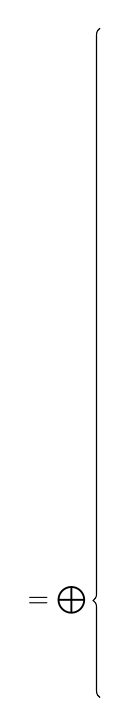
\begin{tikzpicture}
    \draw[decorate,decoration={brace,aspect=0.145}] (0,-8.5) -- (0,0);
    \node[anchor=east,inner sep=0mm] at (-0.15,-7.265) {$= \bigoplus$};
  \end{tikzpicture}%
  \hfill%
  \subcaptionbox{%
    Hierarchical not-a-knot B-splines
    $\bspl[\nak]{l',i'}{p}$ ($l' \le l$, $i' \in \hiset{l'}$)
    and grid points $\gp{l',i'}$ \emph{(dots).}%
  }[71mm]{%
    \includegraphics{hierarchicalBasis_9}%
  }%
  \caption[%
    Nodal and hierarchical not-a-knot B-splines%
  ]{%
    Univariate nodal and hierarchical cubic not-a-knot B-splines ($p = 3$)
    up to level $l = 3$.
    The nodal space $\nsbspl[\nak]{l}{p}$,
    which coincides with the not-a-knot spline space $\naksplspace{l}{p}$,
    decomposes into the direct sum
    of the hierarchical subspaces $\hsbspl[\nak]{l'}{p}$ ($l' \le l$).
    The knots of each level $l'$ are given by removing the
    first $\tfrac{p-1}{2}$ and last $\tfrac{p-1}{2}$
    inner points \emph{(crosses)}
    from the set of grid points $\gp{l',i'}$
    ($i' = 0, \dotsc, 2^{l'}$).%
  }%
  \label{fig:notAKnotBSpline}%
\end{figure}

\vspace*{\fill}

The motivation for using Lagrange polynomials for coarse levels
is that they form a basis of the polynomial space
and that they can be implemented and calculated quickly.
However, the specific choice of basis functions for the levels
$l < \ceil{\log_2(p + 1)}$ is arbitrary,
as long as these functions are linearly independent
(of each other and of the ``true'' not-a-knot B-splines
$\bspl[\nak]{l,i}{p}$, $l \ge \ceil{\log_2(p+1)}$)
and contained in the space $\naksplspace{l}{p}$.

\pagebreak

\paragraph{Implementation}

Note that in each level $l \ge \ceil{\log_2(p+1)}$,
only the first $\tfrac{p+1}{2}$
(indices $i = 1, 3, \dotsc, p$)
and the last $\tfrac{p+1}{2}$
(indices $i = 2^l - p, 2^l - p + 2, \dotsc, 2^l - 1$)
hierarchical basis functions $\bspl[\nak]{l,i}{p}$
differ from $\bspl{l,i}{p}$,
i.e., we have
\begin{equation}
  \bspl[\nak]{l,i}{p} = \bspl{l,i}{p},\quad
  i = p + 2,\; p + 4,\; \dotsc,\; 2^l - p - 2.
\end{equation}

\vspace*{\fill}

\noindent
This means that we can reuse uniform B-spline code
for the inner functions.
Due to $\bspl[\nak]{l,i}{p}(x) = \bspl[\nak]{l,2^l-i}{p}(1-x)$
(because of the symmetry of $\nodalknotseq[\nak]{l}{p}$),
we only have to reimplement $\tfrac{p+1}{2}$ not-a-knot B-splines per level $l$.
As $\bspl[\nak]{l,i}{p}$ and $\bspl[\nak]{l+1,i}{p}$
use the same knots up to an affine transformation for $l$ large enough
($l \ge 3$ suffices for $p = 3$),
only a number of special cases for coarse levels $l$ must be implemented.
In other words, the not-a-knot approach is ``minimally invasive''
with respect to an implementation that already uses uniform B-splines.

\pagebreak

\paragraph{Hierarchical splitting}

The main benefit of the hierarchical not-a-knot B-spline basis
is the validity of the hierarchical splitting.
As usual, we define $\nsbspl[\nak]{l}{p}$ and $\hsbspl[\nak]{l}{p}$
as the nodal and the hierarchical not-a-knot subspace of level $l$,
respectively.

\begin{proposition}[%
  univariate hierarchical splitting for not-a-knot B-splines%
]
  \label{prop:hierSplittingNAKBSplineUV}
  The hierarchical splitting \eqref{eq:hierSplittingUV}
  holds for the hierarchical not-a-knot B-spline basis:
  \begin{equation}
    \naksplspace{l}{p}
    = \nsbspl[\nak]{l}{p}
    = \bigoplus_{l'=0}^l \hsbspl[\nak]{l'}{p},
  \end{equation}
  where for $l < \ceil{\log_2(p+1)}$, $\naksplspace{l}{p}$
  is defined as the space $\polyspace{2^l}$ of polynomials of degree
  $\le 2^l$ on $\clint{0, 1}$.
  (For $l \ge \ceil{\log_2(p+1)}$,
  $\naksplspace{l}{p}$ is the not-a-knot spline space.)
\end{proposition}

\begin{proof}
  For $l < \ceil{\log_2(p+1)}$, all
  three spaces coincide with $\polyspace{2^l}$ and nothing is to prove.
  
  For $l \ge \ceil{\log_2(p+1)}$,
  we check the two conditions of \thmref{lemma:hierSplittingUV}.
  First, the hierarchical subspace $\hsbspl[\nak]{l'}{p}$ ($l' \le l$)
  is a subspace of $\naksplspace{l}{p} = \nsbspl[\nak]{l}{p}$.
  This is a conclusion of \thmref{prop:splineSpace}, as
  every function $\bspl[\nak]{l',i'}{p}$ ($i' \in \hiset{l'}$)
  is continuous on $\clint{0, 1}$, a polynomial on every knot interval of
  $\nodalknotseq[\nak]{l}{p}$, and at the knots themselves
  at least $(p - 1)$ times continuously differentiable.
  
  Second, the hierarchical functions $\bspl[\nak]{l',i'}{p}$
  ($l' \le l$, $i' \in \hiset{l'}$) are linearly independent.
  This can be shown similarly to the proof of
  \thmref{prop:hierBSplineLinearlyIndependent}.
  The linear independence of the Lagrange polynomials
  can be checked by inserting grid points into a zero linear combination.
  The linear combination collapses and only one term remains,
  the coefficient corresponding to the grid point.
  Hence, all coefficients must vanish.
\end{proof}

\vspace*{1em}

\begin{corollary}[%
  multivariate hierarchical splitting for not-a-knot B-splines%
]
  \label{cor:hierSplittingNAKBSplineMV}
  It holds
  \begin{equation}
    \naksplspace{\*l}{\*p}
    = \nsbspl[\nak]{\*l}{\*p}
    = \bigoplus_{\*l'=\*0}^\*l \hsbspl[\nak]{\*l'}{\*p},
  \end{equation}
  where $\naksplspace{\*l}{\*p}$ is the
  tensor product space of $\naksplspace{l_t}{p_t}$
  ($t = 1, \dotsc, d$) as defined in \cref{prop:hierSplittingNAKBSplineUV}.
\end{corollary}

\begin{proof}
  Follows directly from \thmref{prop:splittingUVToMV}.
\end{proof}

\paragraph{Sparse grids with not-a-knot B-splines}

Regular sparse grid spaces using the new hierarchical not-a-knot basis
are defined analogously to the uniform case, i.e.,
\begin{equation}
  \label{eq:sparseGridRegularNAK}
  \regsgspace[\*p,\nak]{n}{d}
  \ceq \bigoplus_{\normone{\*l} \le n} \hsbspl[\nak]{\*l}{\*p}.
\end{equation}
If the level $n$ is large enough, then $\regsgspace[\*p,\nak]{n}{d}$
contains the space $\polyspace{\*p}$ of all $d$-variate polynomials of
coordinate degree $\le \*p$ on $\clint{\*0, \*1}$
(i.e., functions $\objfun\colon \clint{0, 1} \to \real$ of the form
$\objfun(\*x) \ceq \sum_{\*q=\*0}^\*p \interpcoeff{\*q} \prod_{t=1}^d x_t^{q_t}$
with $\interpcoeff{\*q} \in \real$).
This means that in contrast to the uniform B-spline basis,
hierarchical not-a-knot B-splines on sparse grids are able to
replicate global polynomials on $\clint{\*0, \*1}$:

\begin{shortcorollary}[%
  sparse grid with not-a-knot B-splines contains polynomials%
]
  \label{cor:sparseGridRegularNAKPolynomials}
  If $n \ge \normone{\ceil{\veclog_\*2(\*p + \*1)}}$,
  then $\polyspace{\*p} \subset \regsgspace[\*p,\nak]{n}{d}$.
\end{shortcorollary}

\begin{proof}
  Let $\*l \ceq \ceil{\veclog_\*2(\*p + \*1)}$ and $n \ge \normone{\*l}$.
  By \cref{cor:hierSplittingNAKBSplineMV}, we have
  $\bigoplus_{\*l'=\*0}^{\*l} \hsbspl[\nak]{\*l'}{\*p} = \naksplspace{\*l}{\*p}$.
  In addition, all $\*l' \in \natz^d$ with $\*l' \le \*l$ satisfy
  $\normone{\*l'} \le n$ and thus,
  $\bigoplus_{\*l'=\*0}^{\*l} \hsbspl[\nak]{\*l'}{\*p} \subset
  \regsgspace[\*p,\nak]{n}{d}$ by \eqref{eq:sparseGridRegularNAK}.
  We conclude
  $\polyspace{\*p} \subset \naksplspace{\*l}{\*p} \subset
  \regsgspace[\*p,\nak]{n}{d}$, which is the asserted claim.
\end{proof}



\subsection{Modified and Non-Uniform Hierarchical Not-A-Knot B-Splines}
\label{sec:323modifiedNAKBSplines}

\paragraph{Modified hierarchical not-a-knot B-splines}

As for uniform and Clenshaw--Curtis B-splines
(\cref{sec:31standardBSplines}),
it is possible to define a modified version of the
hierarchical not-a-knot B-spline basis to obtain
``reasonable'' boundary values without boundary points.
However, we cannot use \thmref{lemma:marsden} similarly to
\eqref{eq:modifiedBSplineConstruction}:
Due to the removal of knots, there is only a single
not-a-knot B-spline $\bspl[\nak]{l,0}{p}$ left of
$\bspl[\nak]{l,1}{p}$.
B-splines $\bspl[\nak]{l,i}{p}$ with index $i < 0$
would vanish on $\clint{0, 1}$.

While we are therefore not able to construct modified functions
whose second derivative vanishes in a neighborhood of $x = 0$,
we can use $\bspl[\nak]{l,0}{p}$ to let the
second derivative vanish in $x = 0$ itself:
\begin{equation}
  \label{eq:modifiedNotAKnotBSpline}
  \bspl[\nak,\modified]{l,i}{p}(x)
  \ceq
  \begin{cases}
    1,&
    l = 1,\quad i = 1,\\
    \bspl[\nak]{l,1}{p}(x)
    - \dfrac{\deriv[2]{x}{\bspl[\nak]{l,1}{p}}(0)}%
    {\deriv[2]{x}{\bspl[\nak]{l,0}{p}}(0)}
    \bspl[\nak]{l,0}{p}(x),&
    l \ge 2,\quad i = 1,\\
    \bspl[\nak]{l,i}{p}(x),&
    l \ge 2,\quad i \in \hiset{l} \setminus \{1, 2^l - 1\},\\
    \bspl[\nak,\modified]{l,1}{p}(1 - x),&
    l \ge 2,\quad i = 2^l - 1.
  \end{cases}
  \hspace*{-2mm}
\end{equation}
The resulting modified hierarchical not-a-knot B-spline basis
$\bspl[\nak,\modified]{l,i}{p}$ is shown with dashed lines
in \cref{fig:modifiedNotAKnotBSpline}.
As before, we have to implement $\bspl[\nak,\modified]{l,1}{p}$
only for a single level $l$, as modified functions of higher levels
are the same up to an affine parameter transformation.
Note again that for $p \ge 5$, we would have to modify additional
interior B-splines as the interior of their support then extends to the
boundary of $\clint{0, 1}$.
We refrain from doing so to keep the definition
\eqref{eq:modifiedNotAKnotBSpline} simple.

\paragraph{Non-uniform hierarchical not-a-knot B-splines}

The not-a-knot construction is completely independent from the
distribution of the grid points at hand.
Consequently, we can define hierarchical not-a-knot B-splines
for non-uniform distributions.
For instance, to define not-a-knot B-splines for
Chebyshev points (see \cref{sec:314nonUniform}),
we first specify the knot sequence as
\begin{subequations}
  \begin{gather}
    \nodalknotseq[\cc,\nak]{l}{p}
    \ceq (\nodalknot[\cc,\nak]{l,0}{p}, \dotsc,
    \nodalknot[\cc,\nak]{l,m+p}{p}),\quad
    m \ceq 2^l + 1,\\
    \nodalknot[\cc,\nak]{l,k}{p}
    \ceq
    \begin{cases}
      \ccgp{l,k-p},&
      k = 0, \dotsc, p,\\
      \ccgp{l,k-(p+1)/2},&
      k = p + 1, \dotsc, 2^l,\\
      \ccgp{l,k-1},&
      k = 2^l + 1, \dotsc, 2^l + p + 1,
    \end{cases}
  \end{gather}
\end{subequations}
and then define hierarchical not-a-knot Clenshaw--Curtis B-splines as
\begin{subequations}
  \begin{gather}
    \bspl[\cc,\nak]{l,i}{p}
    \ceq
    \begin{cases}
      \lagrangepoly[\cc]{l,i},&
      l < \ceil{\log_2(p+1)},\\
      \nonunifbspl{i,\nodalknotseq[\cc,\nak]{l}{p}}{p},&
      l \ge \ceil{\log_2(p+1)},
    \end{cases}\quad
    l \in \natz,\quad
    i \in \hiset{l},\\
    \lagrangepoly[\cc]{l,i}\colon \clint{0, 1} \to \real,\quad
    \lagrangepoly[\cc]{l,i}(x)
    \ceq \!\!\prod_{\substack{i'=0,\dotsc,2^l\\i'\not=i}}
    \frac{x - \ccgp{l,i'}}%
    {\ccgp{l,i} - \ccgp{l,i'}}.
  \end{gather}
\end{subequations}

This definition can even be combined with the modification
of hierarchical not-a-knot B-splines as discussed above.
We can use exactly the same approach as in
\eqref{eq:modifiedNotAKnotBSpline}, if we replace the
not-a-knot basis functions with their non-uniform not-a-knot counterparts
(not-a-knot Clenshaw--Curtis B-splines in the above example).
The hierarchical not-a-knot Clenshaw--Curtis B-spline basis of
cubic degree and the corresponding modified functions are shown in
\cref{fig:clenshawCurtisNotAKnotBSpline}.

\begin{figure}
  \subcaptionbox{%
    $\bspl[\nak]{l',i'}{p}$,
    $\bspl[\nak,\modified]{l',i'}{p}$
    \emph{(dashed),} and $\gp{l',i'}$ \emph{(dots).}%
    \label{fig:modifiedNotAKnotBSpline}%
  }[73mm]{%
    \includegraphics{hierarchicalBasis_10}%
  }%
  \hfill
  \subcaptionbox{%
    $\bspl[\cc,\nak]{l',i'}{p}$,
    $\bspl[\cc,\nak,\modified]{l',i'}{p}$
    \emph{(dashed),} and $\ccgp{l',i'}$ \emph{(dots).}%
    \label{fig:clenshawCurtisNotAKnotBSpline}%
  }[76mm]{%
    \includegraphics{hierarchicalBasis_11}%
  }%
  \caption[%
    Comparison of hierarchical not-a-knot B-splines%
  ]{%
    Comparison of uniform \emph{(left)} and
    Clenshaw--Curtis \emph{(right)} hierarchical cubic not-a-knot
    B-splines $\bspl[\nak]{l',i'}{p}$ and
    $\bspl[\cc,\nak]{l',i'}{p}$
    ($l ' \le l$, $i' \in \hiset{l'}$, $p = 3$) up to level $l = 3$
    together with the respective modified versions
    $\bspl[\nak,\modified]{l',i'}{p}$ and
    $\bspl[\cc,\nak,\modified]{l',i'}{p}$
    \emph{(dashed).}
    The knots of each level $l'$ are given by removing the
    first $\tfrac{p-1}{2}$ and last $\tfrac{p-1}{2}$
    inner points \emph{(crosses)}
    from the set of grid points $\gp{l',i'}$ or
    $\ccgp{l',i'}$
    ($i' = 0, \dotsc, 2^{l'}$), respectively.%
  }%
  \label{fig:uniformAndClenshawCurtisNotAKnotBSpline}%
\end{figure}



\subsection{Other Approaches to Incorporate Boundary Conditions}
\label{sec:324naturalBoundary}

Not-a-knot boundary conditions are not the only approach
to obtain a subspace of $\wholesplspace{l}{p}$ with the right dimension $2^l - 1$.
Another possibility, which we want to discuss briefly, are
\term{natural boundary conditions.}
In the cubic case, for which they are usually formulated
\cite{Hoellig13Approximation},
these boundary conditions require that the
second derivatives $\deriv[2]{x}{\basis{l,i}}$ of the
basis functions vanish at the boundary $x \in \{0, 1\}$.
To obtain the necessary number of $p - 1$ constraints also
for higher degrees $p$,
we require that all derivatives
$\deriv[q]{x}{\basis{l,i}}$ of order
$q = 2, \dotsc, \tfrac{p+1}{2}$ vanish at $x \in \{0, 1\}$.

%\usenotation{Ënat}
Consequently, we can define hierarchical natural B-splines as
\begin{subequations}
  \begin{gather}
    \bspl[\ntrl]{l,i}{p}(x)
    \ceq
    \begin{cases}
      \lagrangepoly{0,i}(x),&
      l = 0,\\
      \bspl{l,i}{p} +
      \sum_{j \in J_i^{p,\ntrl}} c_{l,i,j} \bspl{l,j}{p},&
      l \ge 1,
    \end{cases}\quad
    l \in \natz,\quad
    i \in \hiset{l},\\
    J_i^{p,\ntrl}
    \ceq \{i-\tfrac{p-1}{2}, \dotsc, i-1\} \cup
    \{i+1, \dotsc, i+\tfrac{p-1}{2}\},
  \end{gather}
\end{subequations}
where the coefficients $c_{l,i,j} \in \real$ are chosen such that
the natural boundary conditions are satisfied:
\begin{equation}
  \deriv[q]{x}{\bspl[\ntrl]{l,i}{p}}(x)
  = 0,\quad
  l \ge 1,\quad
  i \in \hiset{l},\quad
  q = 2, \dotsc, \tfrac{p+1}{2},\quad
  x \in \{0, 1\}.
\end{equation}
The first half of the coefficients $c_{l,i,j} \in \real$
($j < i$) vanishes if the interior of the support of $\bspl{l,i}{p}$
does not contain $x = 0$
(i.e., $i \ge \tfrac{p+1}{2}$).
The second half of the coefficients~($j > i$) vanishes analogously
if $1 \notin \interiorsupp \bspl{l,i}{p} \iff i \le 2^l - \tfrac{p+1}{2}$.
This means that
only the first $\floor{\tfrac{p+1}{4}}$ and the last $\floor{\tfrac{p+1}{4}}$
hierarchical functions have to be altered in each level.

\Cref{fig:naturalBSpline} shows the hierarchical natural spline basis.
The main disadvantage of natural boundary conditions is that
we are not able to replicate arbitrary polynomials exactly on $\clint{0, 1}$
with this approach.
Only polynomials that satisfy natural boundary conditions themselves
(linear polynomials for example)
can be replicated exactly.
For this reason, we do not further consider this basis in the
rest of the thesis.

\begin{SCfigure}
  \includegraphics{hierarchicalBasis_12}%
  \caption[%
    Hierarchical natural B-splines%
  ]{%
    Hierarchical cubic natural B-splines
    \vspace{-0.1em}%
    $\bspl[\ntrl]{l',i'}{p}$
    ($l' \le l$, $i' \in \hiset{l'}$, $p = 3$) and
    \vspace{0.05em}%
    grid points $\gp{l',i'}$ \emph{(dots)} up to level $l = 3$.%
  }%
  \label{fig:naturalBSpline}%
\end{SCfigure}
